\subsection{Pump-induced change in reflectivity}
\label{sec:eval:refl}

We monitor the reflectivity
of the sample during the measurements.
The amount of reflected light
is an important quantity
to estimate the dissipated power $D$ (\ref{eq:dissip}),
which itself is important
in order to asses the heat flow
in the VECSEL device \cite{Heinen2012}.
It turns out,
the reflected fraction
is not constant.
Instead,
it depends on
the incident pump power
and the heat sink temperature.

This observation of reflectivity
was so far not reported
in literature.
In this section
I present the general observations,
followed by a more detailed
analysis of the reflectivity
in the low pump regime --
what I will call base reflectivity.
The section closes
presenting some potential effects
that may contribute
to this phenomenon.

\subsubsection{Observation}

The reflectivity
off the VECSEL structure,
$r=R/P$,
changes depending on
the heat sink temperature
and the pump power.
Figure~\ref{img:basereflectivity}
illustrates this statement.

\begin{figure}
\centering
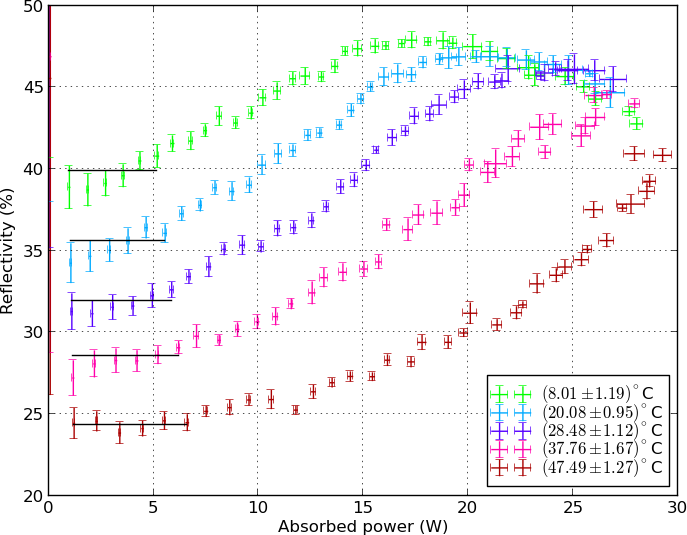
\includegraphics[width=14.5cm]{img/basereflectivity_temperatures.png}
\caption{Sample 1.
The reflectivity
changes depending on pump power
and heat sink temperature.}
\label{img:basereflectivity}
\end{figure}

On the one hand side,
the reflectivity decreases
for an increase
in heat sink temperature.
With higher absorbed power
the temperature
inside the device
increases further.
However,
for higher absorbed power
the reflectivity increases.
Consequentially,
the pump induced change in reflectivity
cannot be a purely thermal effect.

The lasing activity
of the device
potentially affects the reflectivity.
In order to test for this,
I measured
the reflected light
when we remove the output coupler.
Figure~\ref{img:basereflectivity_nooc}
plots three temperatures
measured with
(depicted in Fig.~\ref{img:basereflectivity})
and without the output coupler.

\begin{figure}
\centering
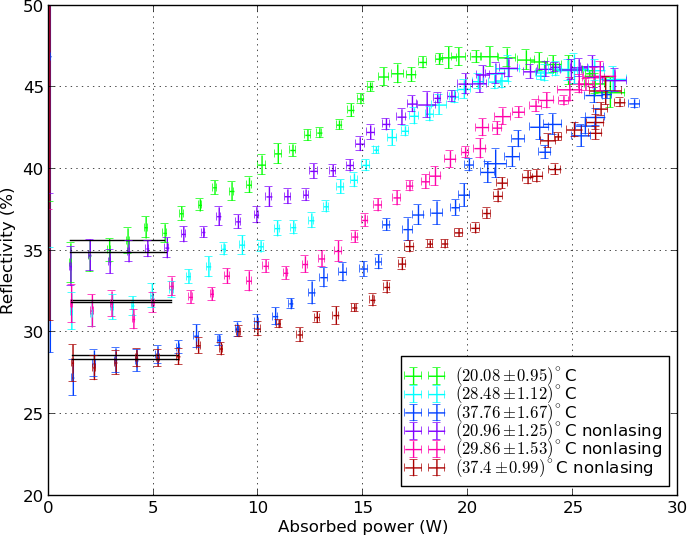
\includegraphics[width=14.5cm]{img/basereflectivity_noOC.png}
\caption{Sample 1.
Reflectivity without output coupler.}
\label{img:basereflectivity_nooc}
\end{figure}

The low pump regime reflectivity
(base reflectivity)
is unaffected
by the presence or absence
of the output coupler.
Increased pump
leads to an increase
in reflectivity;
qualitatively similar
to the lasing configuration.
But,
quantitatively,
this increase is less steep
when we remove the output coupler.

Once the reflectivity has reached
its peak value
it decreases again.
The point of peak reflectivity
does not coincide
with an apparent effect
in the light light performance,
Fig.~\ref{img:LL_sample}.

We have treated sample 1
with an anti-reflectance coating,
in an attempt to investigate
an optimization strategy,
laid out in section~\ref{sec:eval:maxout:AR}.
Figure~\ref{img:refl_sampleAR}
demonstrates the base reflectivity
indeed to be lowered.
The AR coated device
also shows an increase
in reflectivity
for higher pump.


\begin{figure}
\centering
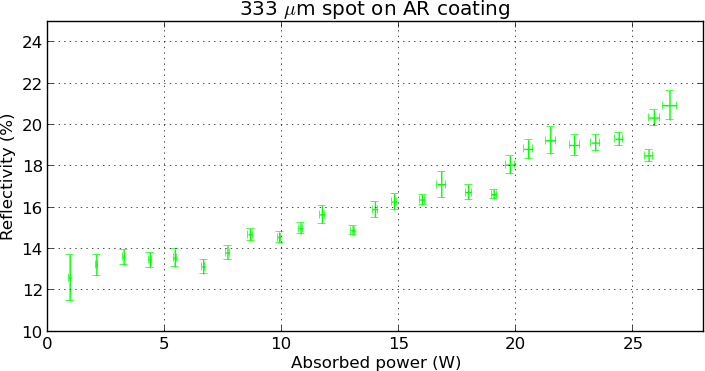
\includegraphics[width=14.5cm]{img/refl_sampleAR.png}
\caption{Sample 1 AR coated.
While the AR coating wasn't successful
to improve the light-light performance,
the base reflectivity indeed was reduced.
The heat sink temperature was
$14.4\pm2.7\,^\circ\mathrm{C}$.
The uncoated sample showed
a base reflectivity of about $38\,\%$
for this temperature.
The coating hence successfully
lowered the reflectivity
to about a third.}
\label{img:refl_sampleAR}
\end{figure}

In Fig.~\ref{img:basereflectivity}--\ref{img:basereflectivity_d6}
the relative reflectivity,
$r=R/P$,
is plotted
against absorbed power $A=P-R$.
A priori
it is not clear
whether this is a good choice.
However,
by doing so
the reflectivity curves
of the different heat sink temperatures
overlap in the decrease regime
after the peak reflectivity.
This overlap
is present for both samples,
and even more apparent
in Fig.~\ref{img:basereflectivity_d6}
of sample 2.
Maybe,
this hints at
an intrinsic limit
of the VECSEL structure.
Plotting $P$ for the x-axis,
the declining line
of the different heat sink temperatures
are shifted with respect to each other.
With $D$ for the x-axis,
the data points corresponding
to the lasing configurations
in Fig.~\ref{img:basereflectivity_nooc}
are shifted left,
such that those
without the output coupler
overshoot the stated line
of decreasing reflectivity.


\subsubsection{Base reflectivity}

For low pump power
the relative reflectivity
shows a flat plateau.
The weighted mean reflectivity
of the regime between 1--$9\,\mathrm{W}$
of pumped power
I call base reflectivity
(the $9\,\mathrm{W}$ is an arbitrary cut,
based on Fig.~\ref{img:basereflectivity}).
This base reflectivity
follows a linear relation
as a function of heat sink temperature.
This is plotted in
Fig.~\ref{img:basereflectivity_fit}
and \ref{img:basereflectivity_d6}
for sample 1 and 2,
respectively.

Sample 2 seems to be about $50\,\%$
more reflective
than sample 1.
Qualitatively,
the increase in reflectance
can be expected.
By reducing the amount
of Ti used
to connect DBR with Au,
the amount of reflected pump light
from this interface
increases \cite{Hader2011}.
This is exactly the difference
between sample 1 and 2,
see section~\ref{sec:basics}.

\begin{figure}
\centering
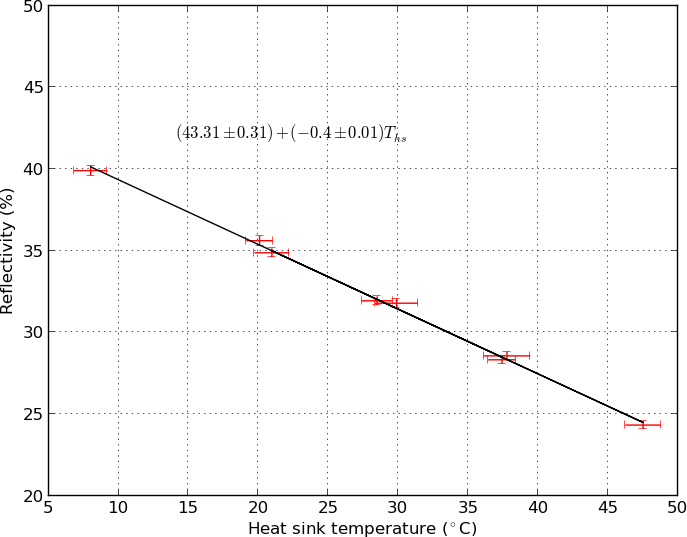
\includegraphics[width=14.5cm]{img/basereflectivity_fit.png}
\caption{Sample 1.
The base reflectivity follows a linear relation
with the heat sink temperature.
The presence of the output coupler
does not affect this low pump regime.
The corresponding measurements
are therefore included.
See Fig.~\ref{img:basereflectivity}
and \ref{img:basereflectivity_nooc}.}
\label{img:basereflectivity_fit}
\end{figure}

\begin{figure}
\centering
\subfigure{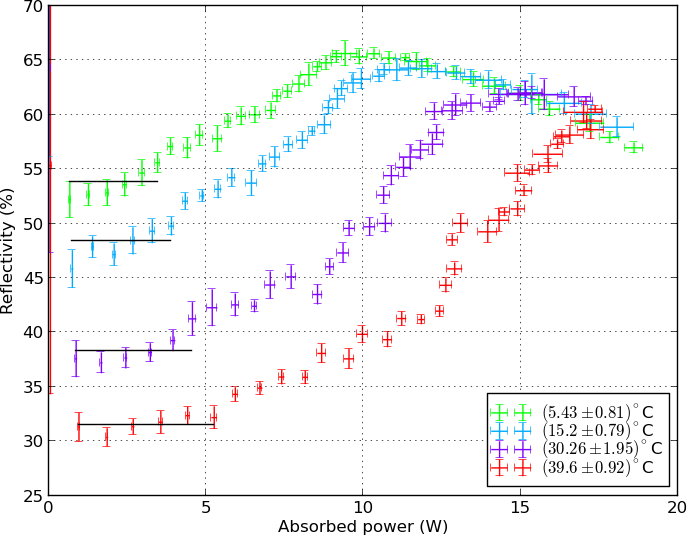
\includegraphics[width=7cm]{img/basereflectivity_temperatures_d6.png}}
\subfigure{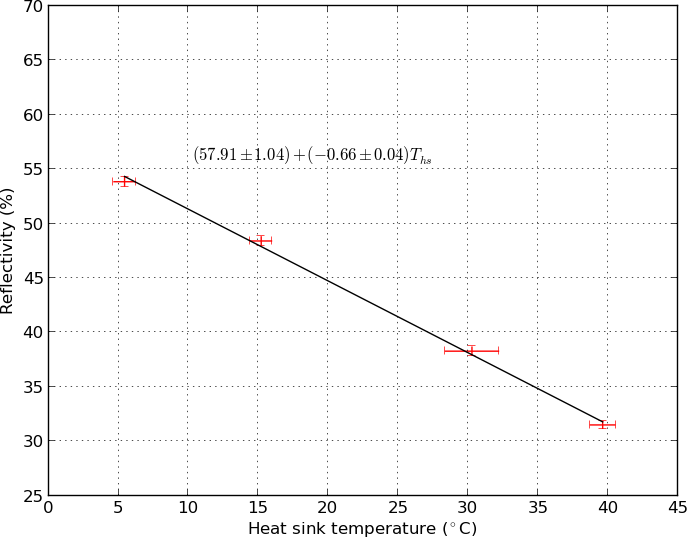
\includegraphics[width=7cm]{img/basereflectivity_d6_fit.png}}
\caption{Sample 2.
The reflectivity
is higher than that for sample 1.
In sample 2 the gold layer
connecting the DBR with diamond
is reflective
while for sample 1,
it absorbs the residual pump.
Compared to Fig.~\ref{img:basereflectivity_fit}
sample 2 is about $50\,\%$
more reflective than sample 1.}
\label{img:basereflectivity_d6}
\end{figure}


\subsubsection{Explanation candidates}

The low pump regime
should be governed
by the simple reflectivity
due to the multi layer nature
of our device.
In order to calculate
this reflectivity value
we need to know
the refractive indices
and absorption coefficients
of all the used AlInGaAs compounds
in our structure.
We don't have access
to such a complete table,
so I cannot calculate this numeric limit. 

Literature
does not provide
a satisfying answer
for this pump induced reflectivity change.
The effect of thermoreflectance
appears to be a related candidate.
It is used for temperature measurements
based on the change in surface reflectivity
\cite{Epperlein1993,Pierscinski2009}.
Accordingly,
the incident pump
perturbes the thermal equilibrium
of the probed structure.
The reflectivity then changes
as a result of this induced modulation.
In semiconductors,
the relationship
between the variation in
optical reflectivity
and temperature
is mainly due to the temperature dependence
of the band gap \cite{Tessier2001},
\begin{equation}
\Delta R = \dd{R}{T} \Delta T.
\end{equation}

The thermoreflectance coefficient $\dd{R}{T}$
varies strongly
with the probed material
and the probe wavelength.
It cannot reliably be simulated numerically,
but has to be determined experimentally
\cite{Pierscinski2009}.
This procedure is time
and equipment intensive.
For this report I omit
determining the thermoreflectance coefficient
of the sample at hand.
Consequentially,
I cannot fit the expected thermoreflectance curve
onto the measured behavior.
And I cannot conclude
whether this concept
leads into the right direction.

The thermal change
in refractive index
is unlikely to be
a relevant contributor
to the pump induced
change in reflectivity:
it depends only weakly on temperature,
$\frac{1}{n_\mathrm{InP}}\frac{\d n_\mathrm{InP}}{\d T}=
2.7(3)\times10^{-5}\,\mathrm{K}^{-1}$
\cite{SpringerMat}.
This change is relevant
for the shift in emission wavelength
and hence section~\ref{sec:rth:lambda}.
But reflectivity
changes in the order of
$R=|\frac{n-1}{n+1}|^2$,
where temperature induced change in $n$
is unlikely to be relevant.

On the other hand,
the barriers are designed to absorb
the incident pump light.
Consequentially,
the temperature dependent band gap change
is of large relevance.

Given the observation
that the change in reflectivity
is not solely a thermal
effect,
we have to assume
there are
(at least)
two different mechanisms
at work.
Motivated by the thermoreflectance,
first,
we attribute
the decrease in base reflectivity
to the band gap of the semiconductor:
As a result of
the elevated temperature
the quantum wells
show a more metallic nature.
Such a structure can absorb
the incident pump
with higher efficacy,
which leaves
less power in the reflection channel.

A second contributing effect
is due to the creation
of electron hole pairs.
By increasing the pump power,
the electron hole pair creation depletes.
At this point
more of the incident light
is not absorbed
and can be reflected
from one of the many layers.

The AR coated sample
showed a decrease
in base reflectivity,
while the uprise
for higher pump power
persisted.
This indicates
the base reflectivity
to be a result
of the many layer structure,
while the reflectivity increase
is due to an internal change.

If the laser emission
is solely relevant
as a cooling channel,
the curves with and without output coupler
should overlap,
when plotted against dissipated power.
However,
with dissipated power,
$D=A-E$,
the data points
from the output coupler configuration
would shift left,
which increases the difference between
the two curves
even more.

Instead,
the explanation
of electron hole pair depletion
expects the reflectivity
to increase faster
in the scenario
the electron hole pairs
are created
due to the stimulated interaction
with the cavity.
In absence of the output coupler
these pairs are still created
because of thermal excitation,
but at a lower rate.
This is what we can see
in Fig.~\ref{img:basereflectivity_nooc}.

Whether my simplistic argument
concerning the bandgap
and electron hole excitation
is tenable,
I leave open
for someone else to discuss.
One objection for example
is that we don't see
an excitation saturation
in the emission measurements.
Secondly,
this explanation
is held very generally
so that
the observed effect
should  appear also in other
VECSEL structures.
I cannot find a publication
describing our observations.

